\documentclass[english, kiv, sem, he, iso690alph, pdf, viewonly]{fasthesis}
\title{Lisp language subset interpret}
\author{Jan}{Hejdušek}
\supervisor{Ing. Kamil Ekštein, Ph.D.}
\assignment{sw2025-02.pdf}

\usepackage{csquotes}
\usepackage{pdfpages}

\nobastardtitle
\nocopyrightnotice

\newif\iffullbuild
\fullbuildfalse

\lstset{style=FASThesisLstStyle, numberblanklines=false, tabsize=5,
keywordstyle=\color{red}}

\begin{document}
\iffullbuild
\frontpages[notm]
\tableofcontents
\fi

\chapter{Introduction}
\section{Overview}
This paper is a documentation for a seminar work in course KIV\slash
PC -- Programming in C language.  I will cover the assignment itself,
analysis of the problem, details of the implementation, short guide
for building and running the application and finally a conclusion
covering how the work went.
\section{Assignment}

The assignment for this seminar work is to develop a console
application in the C~programming language that interprets a subset of
the Lisp programming language (hereafter referred to only as Lisp).
The complete assignment, in Czech, is provided at the end of this document.

\chapter{Analysis}
\section{Problem statement}
As stated, the primary objective is to design and implement an
interpreter for a~subset of Lisp. The interpreter must be capable of
processing source code provided
either in a file or interactively via a command--line interface.

\section{Lisp Grammar}
Our Lisp strictly follows a fully parenthesized prefix notation
(except for a quote) and Expressions in our Lisp can only be either a
constant, list or a
symbol\slash~string identifier, for example:
\lstinline|(1 is a constant and (this is a list of symbols))|.
If we treat operators the same way as variable identificators
we can describe the structure vith a simple context free grammar.
\begin{align*}
  L & \rightarrow EL \mid \epsilon                    \\
  E & \rightarrow\ \texttt{'}E \mid (L) \mid C \mid S \\
  C & \rightarrow \textit{constant}                   \\
  S & \rightarrow \textit{string identifier}
\end{align*}
However by those rules we can also create expressions that are not
part of our Lisp.  Meaning if we parse the source code acording to
this grammar, we will
miss on some syntax errors that will be necessary to catch during evaluation.

We could also design much more complex grammar that could also categhorize
the oparators and function calls, check correct number of arguments and more.
With this we coul find additional syntax errors in the source code,
for example that conditions expexting T or NIL
\footnote{T and NIL are special values use by Lisp to indicate
true\slash~false or an empty list}.
However most of those syntax errors could still happen in runtime due
to nature of variables in Lisp.
Because variables can be passed almost everywhere and can contain any
valid Lisp expression.
Meaning we will have to check for those syntax errors during runtime anyway.

For our purpose, the simple grammar is sufficient enough. With the
tradeof of how easy to parse it is.

\section{Syntax Tree}
We will need to design a data structure capable of representing the
Lisp expressions
that will later be possible to traverse and evaluate. For such
structure there are multiple options:
\begin{enumerate}
  \item \textbf{Binary tree\slash s--expression}: One child
    represents a value of the node
    or contain another node and the other child would work as a
    linked list. See \ref{fig:ast_example2}
  \item \textbf{N--ary tree}: Each node can have an arbitrary number
    of children,
    matching the parenthesis structure. Each list is a node with
    children for each element of the list. See \ref{fig:ast_example}
  \item \textbf{Stack based}: The operands and operators
    could be together
    with parenthesis pushed into a stack and retrieved for each operator.
\end{enumerate}

We will not discuss Stack based evaluation further as it would be
hard to manage loops,
unevaluated parts of the code and quite an overhead would be
necessary to keep track of current operations.
Essentially we would be building our own call stack and the solution
would not be better than other options.

\begin{figure}[h]
  \centering
  \begin{minipage}{0.48\textwidth}
    \centering
    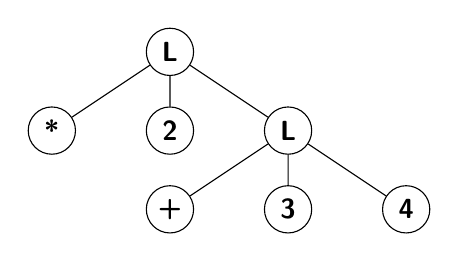
\begin{tikzpicture}[
        every node/.style={draw, circle,minimum size=0.6cm, inner
        sep=0pt,font=\sffamily\bfseries},
      level distance=1cm, ]
      \node {L}
      child { node {*} }
      child { node {2} }
      child { node {L}
        child { node {+} }
        child { node {3} }
        child { node {4} }
      };
    \end{tikzpicture}
    \caption{N--arry syntax tree representing \texttt{(* 2 (+ 3 4))}}
    \label{fig:ast_example}
  \end{minipage}
  \hfill
  \begin{minipage}{0.48\textwidth}
    \centering
    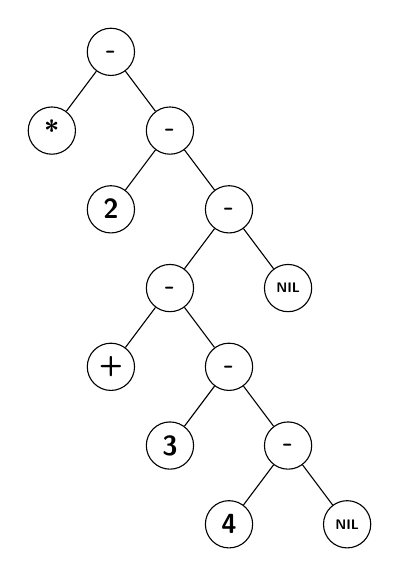
\begin{tikzpicture}[
        every node/.style={draw, circle, minimum size=0.6cm, inner
        sep=0pt, font=\sffamily\bfseries},
      level distance=1cm, ]
      \node {-}
      child { node {*} }
      child { node {-}
        child { node {2} }
        child { node {-}
          child { node {-}
            child { node {+} }
            child { node {-}
              child { node {3} }
              child { node {-}
                child { node {4} }
                child { node {\tiny{NIL}} }
              }
            }
          }
          child { node {\tiny{NIL}} }
        }
      };
    \end{tikzpicture}
    \caption{S--expression syntax tree representing\texttt{(* 2 (+ 3 4))}}
    \label{fig:ast_example2}
  \end{minipage}
\end{figure}

\subsection{S--expression}
Lisp is originally designed with s(symbolic)--expressions in mind as
its internal structure and many of its functionalities are based on it.
Syntax tree represented as an S--expression has few specific features.

Some traversals of the syntax tree are dificult to make, for example
right to left traversal requires either back--links or accumulating children.
Since every list is essentailly a~linked list, access time to its
elements is $O(n)$ where $n$ is index if the elements,
also we do not know the size of the list without going through all the nodes.

The 'NIL' object used in Lisp also appears naturally in the
s--expression as a list terminator.
Also for example the function \lstinline|CDR| returning a list without
the first element is straignhforward to implement as it is just the 'tail' node.

\subsection{N--ary Tree}
N--ary tree is a natural way to represent a nested parenthesized
lists structure and quite universal.
Having all list elements in one array is pleasant to work with and it
is straignhforward to traverse an abstract syntax tree(AST) in any order.
It ouperforms s--expresson in both time and memory for large lists,
$O(1)$ access time to list elements and not using as many nodes.

However for this our purpose, it is not practikal exactly where
s--expression and Lisp behave specifically.
Dynamically allocating arrays and coppying data for the lists is more compplex
than in s--expression where it may be just changing one reference to a node.

The \lstinline|CDR| function requires either having a counter at each node
if it was cdr'd during evaluation and checking it on every other operation
or to create a dummy list node and copy all the remaining references in a list.
With the \lstinline|CDR| function it gets even more complex when we
want to use it for changing content of variables
where we want to replace a whole part of a list with something
else(which is again straignhforward in s--expressions).

Also we would have to artificially create the NIL value,
that does not appear in the structure.

\chapter{Implementation}
\section{Architecture Overview}
The interpreter is divided into several modules:
\begin{itemize}
  \item \textbf{Preprocessor}: Removes comments and normalizes input
  \item \textbf{Lexer}: Tokenizes source code into tokens.
  \item \textbf{Parser}: Converts token array into an AST according
    to the grammar.
  \item \textbf{AST Module}: Utils for creating, copying, and freeing AST nodes.
  \item \textbf{Environment}: Manages variable storage and lookup.
  \item \textbf{Operators}: Implements Lisp functions and
    arithmetic/logical operators.
  \item \textbf{REPL}: Read--eval--print loop
\end{itemize}
See \ref{fig:workflow} for workflow diagram of the program.

\begin{figure}[h!]
  \centering
  \includegraphics[width=.8\textwidth]{img/dataflow.pdf}
  \caption{Interpreter workflow}
  \label{fig:workflow}
\end{figure}

\subsection{Used Data Dtructures}
\subsubsection{AST node}
The AST node uses a union to store data for different node types:
numbers and booleans use an integer \lstinline|value| field, symbols
use contain a \lstinline|char*| in \lstinline|symbol|,
and lists contain a reference array of child nodes together with
child count.

The \lstinline|node.type| field determines which union
member is valid. For example a first node in a list can be accessed
vith \lstinline|node.as.list.children[0]|

Lastly the \lstinline|node.origin| field is used for memory
management marking if the
node is temporary used to pass evaluation results, variable or a part
of the original AST. See \ref{src:astnode} for C source code.

\newpage

\begin{code}{C}{AST node struct\label{src:astnode}}
  typedef struct ASTnode {
    enum node_type {
      BOOLEAN,
      NUMBER,
      SYMBOL,
      LIST,
    } type;
    enum node_origin {
      UNSET,
      AST,
      VARIABLE,
      TEMPORARY,
    } origin;
    union {
      int value;
      char *symbol;
      struct {
        struct ASTnode **children;
        int count;
      } list;
    } as;
  } astnode;
\end{code}

\subsubsection{Operators}
Looking up the correct C functions for each Lisp operator(by operators
  also refering
to Lisp functions) is done using a \lstinline|struct operator_entry|
which maps a string to a function. We keep an entry for each operator
in an array \lstinline|operators|.

\subsubsection{Environment variables}
Variables are stored as pairs of string(name of the variable) and
\lstinline|ASTnode| struct inside an array contained in
\lstinline|Env| together with count of existing variables. See
\ref{src:env} for C source code.

\begin{code}{C}{Environment struct\label{src:env}}
  struct var_record {
    char *symbol;
    astnode *node;
  };

  typedef struct Env {
    struct var_record *vars;
    int var_count;
  } env;
\end{code}

\section{Macros and Error handling}

Throughout the entire source code macros are videly used for error
handling, returning \lstinline|enum err_t| from functions.
See \ref{src:macros} for demonstration of how the macros are used.
The are currently 5 macros in use:
\begin{enumerate}
  \item \lstinline|RETURN_ERR_IF(cond, err)|
  \item \lstinline|RETURN_VAL_IF(cond, retval)|
  \item \lstinline|RETURN_NULL_IF(cond)|
  \item \lstinline|CLEANUP_WITH_ERR_IF(cond, label, err)|
  \item \lstinline|LOG_IF_VERBOSE(err)|
\end{enumerate}

The first 3 macros simply return given value, respectively NULL or an
error if the condition passes. \lstinline|CLEANUP_WITH_ERR_IF| macro
additionally jumps to label and sets variable retval to given err
instead of returning it. \lstinline|LOG_IF_VERBOSE(err)| macro is
used inside the macros, further described in \ref{sec:errorlog}

\newpage
% tex-fmt: off
\begin{code}{C}{Common function structure returning \lstinline|err_t|\label{src:macros}}
  err_t func(args) {
    /* sanity check */
    RETURN_ERR_IF(sanity_condition, ERR_INTERNAL);

    err_t err, retval = ERR_NO_ERROR;

    /* code that possibly allocs */

    CLEANUP_WITH_ERR_IF(early_return_condition, cleanup, ERR_NO_ERR);

    err = func_that_can_fail();
    CLEANUP_WITH_ERR_IF(err, fail_cleanup, err);

    cleanup:
    free(stuff_to_free_on_success);
    return retval
    fail_cleanup:
    free(sutff_to_free_on_falilure);
    return retval
  }
\end{code}
% tex-fmt: on

\subsection{Error logging}
\label{sec:errorlog}
The added value over putting the code into \lstinline|if(cond){/* code */}|
, is firstly increased readability and the ability to log
file name and line number when errors occur. Meaning that if we keep this
structure throughout the code, we can print the entire call stack
when an error is caught, which can greatly reduce time debugging the
code.

This logging is done by the last used macro
\lstinline|LOG_IF_VERBOSE(err)| that prints the error message to
\lstinline|stderr| stream and any subsequent calls append to this
print. If we do not want to generate all the code for logging the
errors, we can turn it off via a compile--time switch, it can greatly
reduce size of the final executable.

\section{Handling Input}
The interpreter supports two modes of input: reading from a file or
interactively from the command line. The mode is determined by
the command-line arguments provided at startup.

\subsection{Arguments}
The first argument of the file is alwais interpreted as a filename, it reads
the entire contents of the file into a buffer.
Optionally, a \lstinline|-v| flag can be provided as a second argument
to enable verbose output, printing the result of each evaluated
expression. 

The argument parsing logic only checks for valid combinations
and prints usage help if the arguments are invalid. Finally the
buffer is passed to the evaluation pipeline for processing, which is
further handled by \lstinline|process_code_block| function.

\subsection{REPL}
If no argument is provided, the program enters an interactive
Read-Eval-Print Loop. In this mode, the interpreter repeatedly
prompts the user for input, reading lines from \lstinline|stdin|.
It accumulates lines until all parentheses are balanced, allowing for
multi-line expressions. 

Once a complete expression is entered, it is
passed into \lstinline|process_code_block| function and essentially
treated in a same way as a source code from a file.
The REPL continues until either
evaluation of a \lstinline|(quit)| expression or an error occured
during evaluation and exits.

\section{Evaluation Pipeline}
\subsection{Preprocessor}
\subsection{Lexer}
\subsection{Parser}
\subsection{Evaluation}
\subsubsection{Environment}
\subsubsection{Operators}

\section{Memory Management}

\chapter{User guide}
\chapter{conclusion}
\iffullbuild
\appendix{}
\chapter{}
\label{assignment}
\includepdf[pages=-]{sw2025-02.pdf}
\fi
\end{document}
